\documentclass[journal,a4paper,pdftex]{lib/IEEEtran}

\usepackage{acronym}
\usepackage[latin1]{inputenc}
\usepackage[italian]{babel,varioref}                    % gestione lingua
\usepackage{amsmath}
\usepackage{amssymb}
\usepackage{multicol}
\usepackage[dvips]{graphicx}

\renewcommand{\acffont}[1]{\textsl{#1}}
\newcommand{\quotes}[1]{``#1"}
\newcommand{\abs}[1]{|#1|}
\newcommand{\eng}[1]{\emph{#1}} 

\pagestyle{empty}

\title{\textit{Ricostruzione traccia audio
    attraverso la scansione di dischi ``Shellacc''
    }\\ \vspace{0.2cm} \small{Corso di Informatica per la
    Cultura, Prof. Giovanni de Poli
%Dipartimento di
%    Ingegneria dell'Informazione, Universit� degli Studi di Padova
		\\a.a. 2010-2011 } }

% XXX Inserite matricola e controllate email
\author{\authorblockN{
Bonetto Riccardo (-IF),
Brundo Salvatore (-IF),
Carlesso Enrico (586563-IF),
Tubiana Mauro (-IF)}\\
        \authorblockA{Dipartimento di Ingegneria dell'Informazione -- Universit� degli Studi di Padova -- Italia \\
                     \texttt{ \small(bonetto, brundosa, carlesso, tubianam)@dei.unipd.it } } }
\begin{document}
\maketitle
% Spazio alle sezioni che dobbiamo scrivere
\section{Introduzione}
\begin{figure}[h!t]
\begin{center}
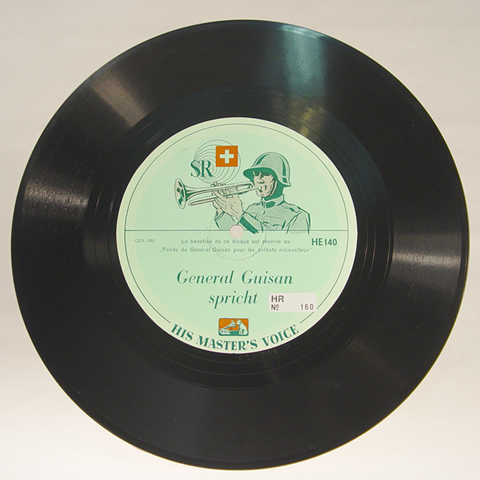
\includegraphics[scale=0.3]{./img/shellac.jpg}
\caption{Disco in gommalacca}
\end{center}
\end{figure}
I dischi di gommalacca (altres\`i noti come \emph{Shellac}) furono il supporto primario per registrazioni musicali estinate al grande pubblico durante tutto il periodo che va dal primo decennio del '900 fino ai tardi anni '50.

Il problema pi\`u frequente che si incontra nella gestione di tali dischi \`e la grande facilit\`a di rottura dovuta alla fragilit\`a intrinseca del materiale
\begin{figure}[h!t]
\begin{center}
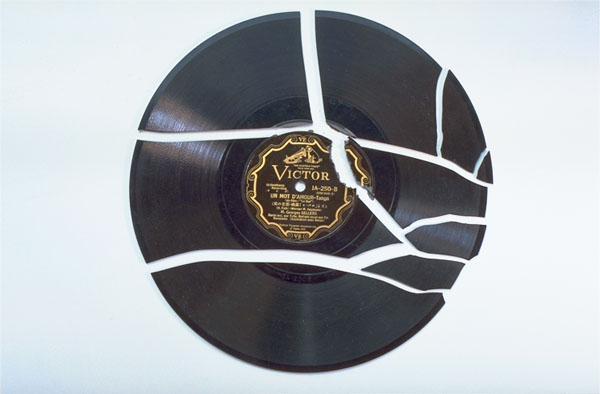
\includegraphics[scale=0.4]{./img/broken_disc.jpg}
\caption{Disco in gommalacca rotto}
\end{center}
\end{figure}
 e, dal momento che molte incisioni su Shellac sono opere uniche e che la loro riproduzione richiede strumenti molto costosi o obsoleti (rischiando quindi di danneggiare il supporto delle incisioni), risulta evidente la necessit\`a di un sistema efficiente di recupero dell'informazione ivi contenuta al fine della sua preservazione e della possibilit\`a di diffusione.
% sezione introduttiva, consegna, scopo
L'obiettivo del progetto \emph{TONI} (\emph{T}he s\emph{O}und i\emph{N} a beam of l\emph{I}ght) \`e la verifica dello stato dell'arte nell'estrazione di segnale audio da una scansione di dischi in gommalacca.

Nel seguito di questa trattazione verr\`a presentato lo studio di un progetto sviluppato presso la Princeton University da Mark McCann, Paul Calamia e Nir Ailon, che anticipava interessanti risultati nel recupero di un segnale audio, verranno quindi analizzate le debolezze di tale lavoro e tratte alcune conclusioni sulle reali possibilit\`a applicative di tale processo.

% XXX Fa sempre bene ricordarsi come si inserisce un'immagine
% 
% \begin{figure}[h!t]
% \begin{center}
% \includegraphics[scale=0.3]{../img/schema_generale.pdf}
% \caption{Schema generale di funzionamento}
% \end{center}
% \end{figure}
% 

\section{Workflow}
% Workflow teorico del processo
L'impostazione teorica del processo di digitalizzazione dell'informazione sonora contenuta nei dischi shellac si articola su quattro fasi principali:
\begin{itemize}
	\item scansione
	\item image processing
	\item sound extraction
	\item filtering
\end{itemize}
\begin{figure}[h!t]
\begin{center}
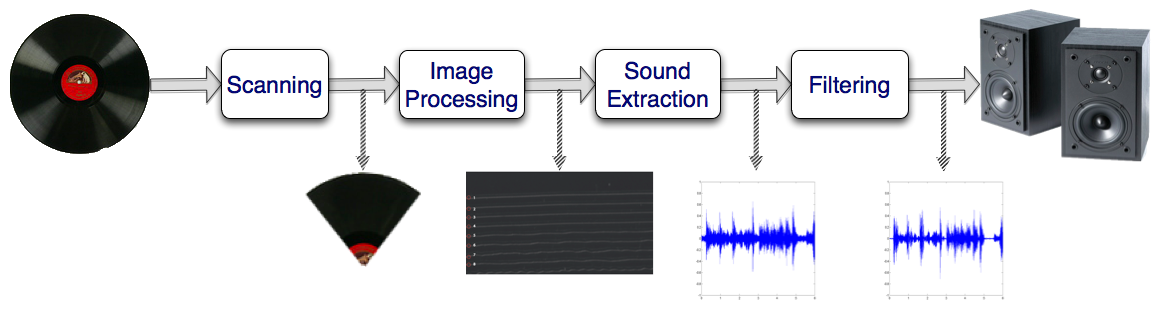
\includegraphics[scale=0.2]{./img/block-scheme.png}
\caption{Workflow generale}
\end{center}
\end{figure}
\subsection{Shellac}
I dischi in gommalacca, seppur soggetti a variazioni dovute ai diversi produttori e periodi di produzione, evidenziano delle caratteristiche il pi\`u delle volte comuni:
\begin{itemize}
	\item diametro tra gli 8 e 12 pollici
	\item massima escursione possibile del solco: 0.15 mm
	\item banda teorica: da 30 Hz 1.6 kHz
	\item banda reale: da 500 Hz a 3.5 kHz
\end{itemize}
Un primo problema che affligge il processo in questione pu\`o, anche intuitivamente, essere dedotto dall'osservazione della massima escursione possibile del solco: 0.15 mm, in poco pi\`u di un decimo di millimetro \`e infatti contenuta tutta l'informazione sonora che si vuole digitalizzare, di conseguenza la risoluzione dell'immagine ottenuta attraverso il processo di scansione dev'essere sufficientemente alta da poter recuperare il preciso andamento dei solchi.

\subsection{Scansione}
La fase di scansione permette di ottenere l'immagine delle tracce che verr\`a in seguito processata.
\begin{figure}[h!t]
\begin{center}
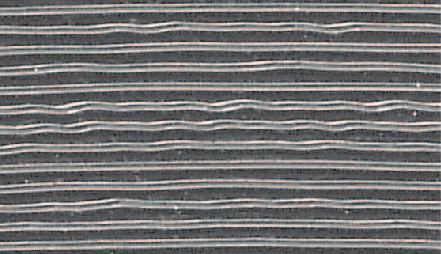
\includegraphics[scale=0.6]{./img/shellac-track.png}
\caption{Porzione di tracce}
\end{center}
\end{figure}
Ottenere un'immagine sufficientemente dettagliata da essere usata negli step successivi di elaborazione si \`e rivelata la fase pi\`u aleatoria dell'intero processo, il livello qualitativo \`e infatti inficiato da svariati fattori derivanti dallo scanner utilizzato e dal posizionamento del disco stesso sul piano del dispositivo.

Dai risultati sperimentali di questa fase \`e emersa la necessit\`a di utilizzare una risoluzione di scansione di 2400 dpi ottici (cio\`e non derivanti da interpolazione software operata dal driver dello scanner) e di rilevare - per ogni scanner utilizzato - il punto di illuminazione ottimale al fine di determinare la porzione di informazione contenente la maggior quantit\`a possibile di informazione.

Il punto di illuminazione ottimale \`e risultato ampiamente variabile a seconda del modello di scanner utilizzato determinando, di conseguenza, la necessit\`a di intraprendere un processo di calibrazione tutte le volte che risulti necessario cambiare dispositivo.

\subsection{Image processing}
La fase di image processing si articola in tre passaggi fondamentali:
\begin{itemize}
	\item ricerca del centro
	\item unwrap dell'immagine
	\item crop dell'immagine
\end{itemize}

\subsubsection{Ricerca del centro}
\begin{figure}[h!t]
\begin{center}
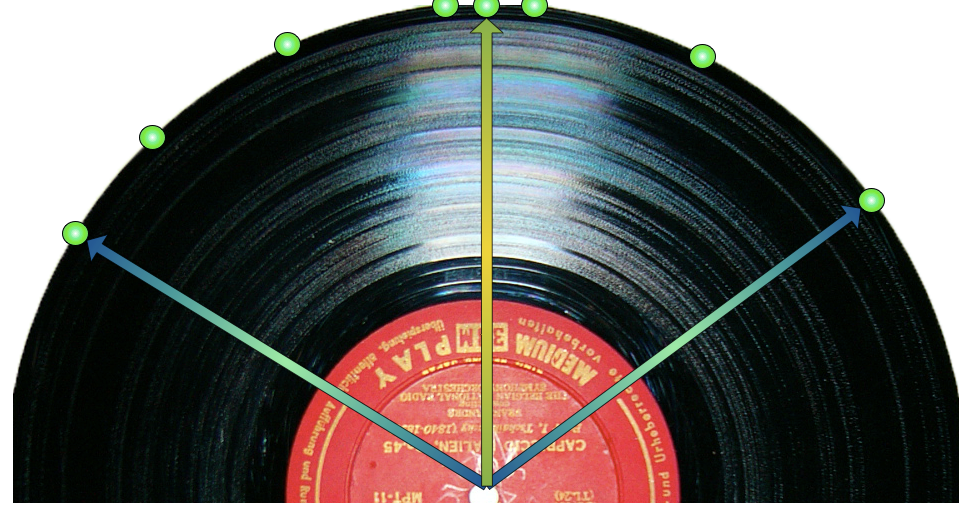
\includegraphics[scale=0.15]{./img/center.png}
\caption{Ricerca del centro}
\end{center}
\end{figure}
La determinazione del centro del disco scannerizzato \`e necessaria alla successiva trasformazione da coordinate cartesiane a coordinate polari che permette di ``raddrizzare'' le tracce.

La detection del centro ha inizio con la determinazione dei bordi del disco sulla base della variazione di luminosit\`a tra lo sfondo dell'immagine (bianco) e la porzione di disco acquisita tramite scansione (sensibilmente pi\`u scura).
Una volta acquisito un numero $N$ di coppie di punti $(x_i,y_i)$ giacenti sul bordo del disco, siano $(x_c, y_c)$ le coordinate del centro e $r$ il raggio del disco, si procede alla soluzione dell'equazione:
$$(x_i-x_c)^2+(y_i-y_c)^2=r^2 \quad i=1,2,\ldots,N$$
che pu\`o essere riscritta come:
$$r^2-x_c^2-y_c^2+2x_cx_i+2y_cy_i = x_i^2+y_i^2$$
e ponendo:
$$
\begin{cases}
a_1= r^2 - x_c^2 - y_c^2\\
a_2 = 2x_c\\
a_3 = 2y_c\\
\end{cases}
$$
si ottiene la forma matriciale:
$$
\begin{pmatrix}
1 && x_1 && y_1\\
1 && x_2 && y_2\\
\vdots && \vdots && \vdots\\
1 && x_N && y_N
\end{pmatrix}
\begin{pmatrix}
a_1 \\
a_2 \\
a_3
\end{pmatrix}
$$
$$
=
\begin{pmatrix}
x_1^2+y_1^2\\
x_2^2+y_2^2\\
\vdots \\
x_N^2+y_N^2
\end{pmatrix}
$$
che, risolta per mezzo del metodo di eliminazione di Gauss-Jordan, fornisce i parametri della circonferenza esterna del disco in esame:
$$
\begin{cases}
	x_c ={a_2\over{2}} \\
	y_c = {a_3\over{2}}\\
	r = \sqrt{x_c^2+y_c^2 + a_3}\\
\end{cases}
$$
\subsubsection{Unwrap}
Una volta determinato il centro del disco, si procede al ``raddrizzamento'' delle tracce per mezzo della trasformazione da coordinate cartesiane a polari:
\begin{figure}[h!t]
\begin{center}
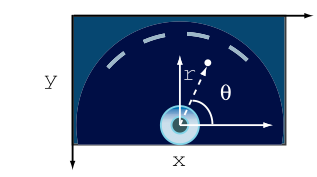
\includegraphics[scale=0.5]{./img/cartesio.png}
\caption{Rappresentazione in coordinate cartesiane}\label{cartesio}
\end{center}
\end{figure}

\begin{figure}[h!t]
\begin{center}
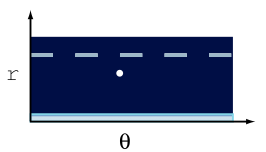
\includegraphics[scale=0.5]{./img/polare.png}
\caption{Rappresentazione in coordinate polari}
\end{center}
\end{figure}
Sia $v(x,y)$ un punto dell'immagine in coordinate cartesiane, la sua trasformazione in coordinate polari sar\`a: $u(r,\theta) = v(x_c+rcos(\theta), y_c+rsin(\theta))$, dove $r$ e $\theta$ sono definiti in figura \ref{cartesio}
\subsubsection{Crop}
Il cropping elimina parti non necessarie dell'immagine, come per esempio quelle relative all'etichetta, in modo da ottenere un file di
\begin{figure}[h!t]
\begin{center}
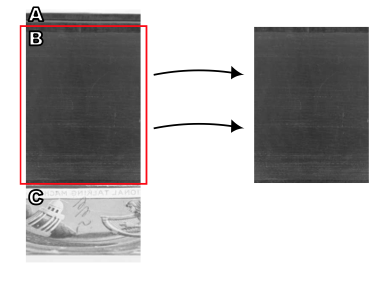
\includegraphics[scale=0.6]{./img/cropping.png}
\caption{Esempio di cropping}
\end{center}
\end{figure}
 dimensioni minori contenente solo l'informazione necessaria al processo.
\subsection{Sound extraction}

\subsubsection{Ricerca delle tracce}
Una volta determinato il centro e croppata l'immagine si prosegue alla localizzazione delle tracce ed al loro inseguimento.

Ogni immagine derivante da scansione viene memorizzata in forma matriciale 
$$I(h,w) = \begin{pmatrix} 
	I(1,1) && \ldots && I(1,w) \\
	\vdots && \vdots && \vdots \\
	I(h,1) && \ldots && I(h,w)
\end{pmatrix}$$  $$I(h,w) \in \{0, 1,2,\ldots, 255\}$$
L'algoritmo di localizzazione fa affidamento sul fatto che i pixel appartenenti a tracce risultino molto pi\`u luminosi rispetto agli altri, quindi sommando i pixel relativi alle righe di $I(h,w)$ (facendo quindi variare l'indice di colonna) si avranno dei picchi in corrispondenza delle tracce (righe).
\begin{figure}[h!t]
\begin{center}
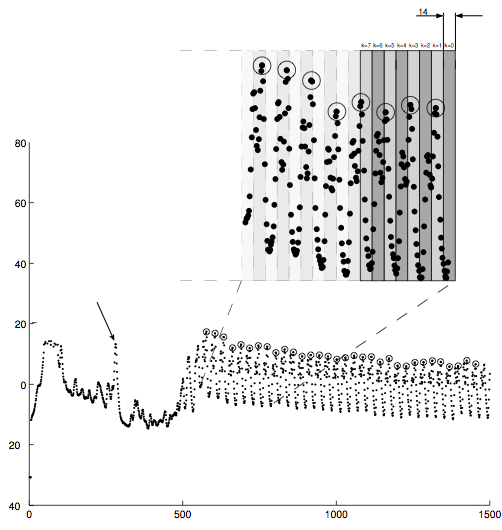
\includegraphics[scale=0.3]{./img/track-detection.png}
\caption{Picchi generati dall'algoritmo di localizzazione}
\end{center}
\end{figure}
\subsubsection{Inseguimeno delle tracce}
La conoscenza dei punti iniziali delle tracce nell'immagine scansionata permette il loro inseguimento per mezzo di un algoritmo euristico ad hoc.

Innanzitutto un vettore di 5 pixel di altezza viene centrato sul punto iniziale della traccia da seguire:
$$
P = 
\begin{pmatrix}
M(y_1+r(0), c)\\
\vdots \\
M(y+1+r(4), c)
\end{pmatrix}
$$
dove $r(i) \in \{-2,-1,0,1,2\}$ e c \`e l'indice di colonna.

Questi valori sono poi usati come pesi per il calcolo del centro di massa del vettore (corrispondente alla posizione della traccia relativamente alla colonna in cui quest'ultimo \`e stato posto): $\rho(n) = {\sum_{i=1}^{5}{P(i)r(i)}\over{\sum_{i=1}^{5}{P(i)c}}}$
\begin{figure}[h!t]
\begin{center}
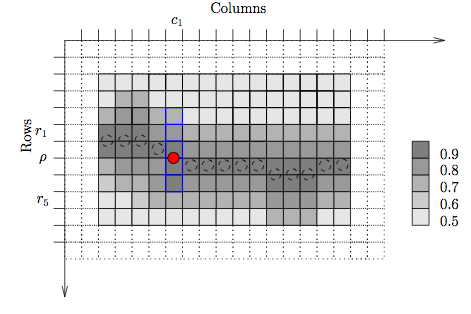
\includegraphics[scale=0.5]{./img/track-following.png}
\caption{Inseguimento delle tracce}
\end{center}
\end{figure}
Ad ogni passo dell'algoritmo il vettore di 5 pixel viene spostato in avanti di una colonna e ne viene determinato il centrodi massa.
\subsubsection{Concatenazione delle tracce}
\begin{figure}[h!t]
\begin{center}
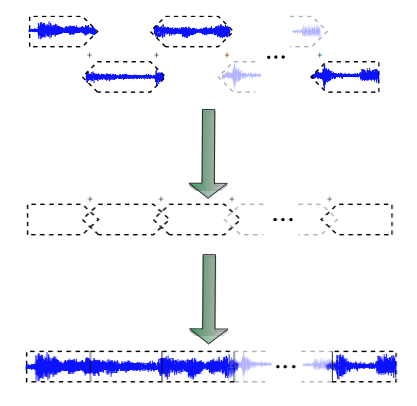
\includegraphics[scale=0.4]{./img/concatenation.png}
\caption{Concatenazione delle tracce}\label{fading}
\end{center}
\end{figure}
Una volta ottenuti gli spezzoni ti tracce da ogni singola immagine, questi devono essere concatenati in modo da ricostruire il brano originale. Una spiegazione grafica di questo processo \`e offerta in figura \ref{fading}
\section{Il progetto analizzato}
L'analisi del progetto sviluppato presso la Princeton University da Mark McCann, Paul Calamia e Nir Ailon si \`e articolata in quattro fasi:
\begin{itemize}
\item Analisi del codice Matlab
\item Creazione del flusso di lavoro
\item Associazione tra flusso del codice e modello teorico
\item Debugging e refactoring del codice
\end{itemize}
\subsection{Analisi del codice ed estrapolazione del flusso di lavoro}
%%manca la parte sul matlab
\section{Conclusioni}
Nel trarre le conclusioni riguardo questo lavoro, appare opportuno scindere esplicitamente i due aspetti analizzati: l'applicabilit\`a ed efficacia teorica del processo di acquisizione ed elaborazione e l'implementazione specifica presa in esame.
\subsection{Efficacia del modello teorico}
Il modello teorico su cui si basa l'approccio studiato sembra essere promettente. Esso infatti permette l'archiviazione in formato digitale di materiale audio, spesse volte unico, per mezzo di una procedura rigorosa e ben documentata che richiede all'utente solamente la disponibilit\`a di uno scanner flatbed ampiamente disponibile nei comuni canali commerciali., rendendo di fatto accessibile al grande pubblico la conservazione di materiale d'epoca.

Nonostante l'apparenza iniziale, tuttavia, analizzando nel dettaglio il processo sono state scoperte diverse insidie (quali per esempio la necessria determinazione del punto di illuminazione ottimale e la procedura intrinsecamente euristica di rilevazione delle tracce) che, di fatto, limitano la fruibilit\`a di questo approccio ad un'utenza con un grado di esperienza medio alto. 

Importante \`e inoltre notare che la necessit\`a di immagini ad alta risoluzione e il processo di elaborazione matriciale necessario all'estrapolazione dell'informazione sonora, richiedono, di fatto, una potenza computazionale non indifferente, limitando ulteriormente la fruibilit\`a di un possibile sistema basato su questo modello teorico ai possessori di architetture hardware di alta fascia.

\subsection{Efficacia dell'implementazione}
L'implementazione fornita dal gruppo della Princeton University \`e risultata essere, a differenza di quanto dichiarato dagli sviluppatori, in uno stadio fortemente prototipale.

I problemi evidenziati nella trattazione precedente rendono il progetto interessante unicamente dal punto di vista accademico e non rendono certo auspicabile una sua diffusione su ampia scala.\\
\`E inoltre interessante notare come i risultati ottenuti in fase di testing del progetto si discostino di molto dai risultati dichiarati dagli sviluppatori. Il file audio ottenuto risulta infatti, anche sotto l'aspetto dell'analisi spettrale, privo di qualunque informazione sonora e di conseguenza inutilizzabile anche nell'eventualit\`a di sofisticati filtri di rimozione del rumore e soun enhancement.

\subsection{Sviluppi futuri}

\vfill

% La bibliografia la caghiam fuori alla brutta
% con thebibliography

\begin{thebibliography}{1}

% XXX Si, ci va prima il nome e poi il titolo.
% Ci pensiam poi
\bibitem{light-blue1} \emph{Final Report}:
  Group light-blue Digiital needle
% \bibitem{opencv} \emph{OpenCV Library}:
%   http://opencvlibrary.sourceforge.net/
% \bibitem{gsl} \emph{GNU Scientific Library}: a numerical library for C
%   and C++ programmers
% \bibitem{hess} \emph{Hess, R., Sift Feature Detector}: A C implementation of a
%   SIFT image feature detector, http://web.engr.oregonstate.edu/~hess/index.html
% \bibitem{tinyOS}
%   \emph{http://www.tinyos.net/tinyos-2.x/doc/}: \texttt{API and
%     Tutorial NesC}
% \bibitem{lowe99} \emph{Lowe, D. G., "Object recognition from local
%   scale-invariant features,"}: \texttt{Proceedings of International
%   Conference on Computer Vision, 1999, pp. 1150-1157}
% \bibitem{lowe04} \emph{Lowe, D. G., "Distinctive Image Features from
%   Scale-Invariant Keypoints"}: \texttt{International Journal of
%   Computer Vision, 2004}
\end{thebibliography}

\onecolumn
\clearpage
% -*- coding: utf-8 -*-
\section{Appendice}
\subsection{Informazioni tecniche sul supporto}
% Dati tecnici sul disco. Quote e bubbole

Eh, niente, il disco \`e tondo e gira.

\clearpage



\end{document}

